\section{Project Description}

Cloud providers operate a huge amount of physical servers. Each server hosts
one to many virtual machines for one or multiple customers, with changing
specifications (mostly amount of allowed RAM, CPU time and storage capacity).
Most providers use over-commitment on the hosts. From time to time bottlenecks
occur because the mixed calculation isn’t perfect and in most cases not
optimized for a single host.

The companies have a placement algorithm which finds a suitable host if
somebody requests a new virtual machine. These algorithms often are very
simple (for example only check the amount of free RAM) and are unable to
achieve a high packing density.

Many service providers still do not have a proper accounting for compute
resources used by a single customer (or even a single instance). This leads to
two issues:
\begin{outline}
  \1 A customer has no vendor-provided visualization of his used and
  available resources.
  \1 The provider can not use resource-based billing which would make him more
  attractive for many use cases.
\end{outline}

The goal of this project is to create a working open source solution that is
capable of resolving the above mentioned issues. Our idea is divided into
three parts:
\begin{enumerate}
  \item Collect all the needed information from each virtual instances on the
    host system, spool them and then send them periodically to the database
    system.
  \item Set up a suitable database software which is scalable and provides a
    certain level of redundancy.
  \item Provide a web interface where customers can see visualizations of their
    utilized resources. Also an API is needed to present the data to different
    kinds of users. A user story survey for the three types of users (customer,
    administrator, manager) will be made at different partners. This will help
    the project team to figure out multiple different algorithms that need to
    be implemented in the API.
\end{enumerate}

There are already several open source software projects that claim to provide a
solution for one of our three points. We will test how well each of them can
work together with other projects until we have found solutions for all listed
points. Scalability is also important: we work together with partners that
operate several 10.000 virtual instances, so we will run benchmarks to create a
solution that is capable of dealing with at least 10.000 instances and still can
scale further. The database setup will be similar to that of a data warehouse,
which will allow us to build and execute complex queries. This should also
provide us with the needed scalability features.

\section{Output}

The customer gets a better overview of the usage behavior from today or a
month, so he can improve the management of his products. The server
administrator can optimize operations by e.g.:
\begin{outline}
  \1 determining if a host system is overloaded and a virtual instance has to
  be migrated to another server. This increases the available performance per
  instance. This will increase the customer satisfaction without the need to
  upgrade the hardware platform.
  \1 determining which host system is the best for new customers.
  \1 determining if new acquisitions of hardware are required.
  \1 determining if the current hardware is overbooked and needs a hardware
  refresh.
\end{outline}

The marketing can use this data for e.g.:
\begin{outline}
  \1 creating upselling campaigns
  \1 giving inactive customers a special offer with lower rates
  \1 new products, like a “pay-per-use” price plan for customers. This can lead
  to a market advantage compared to other providers in this branch.
\end{outline}

\section{Possible negative side effects}

It is possible that we create a denial of service attack against the network
infrastructure when several thousand hypervisors send logs of all running
virtual machines to our data storage system. We have to safely calculate and
test the amount of bandwidth needed and monitor the usage to prevent a DoS.
Data pushing versus pulling are two fundamentally different concepts, it is
easily possible to overextend the database if the wrong technology is used
here. Maybe we need to set up a queues in front of the database to handle the
load and to have a single entry point to the data storage system.


\section{Quality Management}

For the quality management and quality assurance, many techniques and tools
will be used from the Continuous Integration (CI) and Continuous Delivery (CD)
principles. Continuous Integration helps the developer to get feedback quickly
about his changes. Each change will trigger a predefined test matrix. When the
tests complete successfully, the working software can automatically be deployed
to different test- and productive environments. An acceptance test of the user
interface (Web-UI and API) through a group of test users will be done for each
milestone. The continuous execution of automated tests lowers the amount of
time needed in dedicated test phases during the project. This allows us to
spend a higher amount of time on the acceptance tests with real persons.

\section{Quality Requirements}
\centering
\raisebox{-5cm}{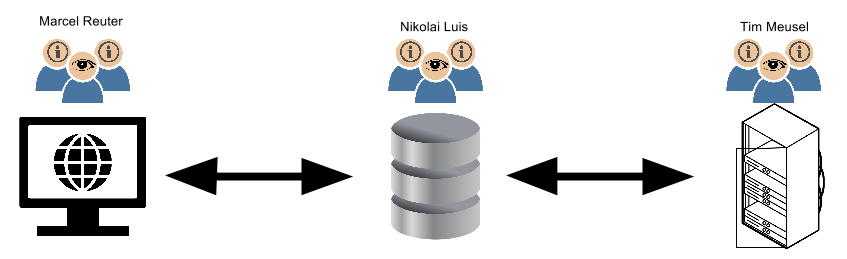
\includegraphics[width=\textwidth]{roles.png}}
\\[1.5cm]
\small
\makebox[\textwidth]{%
    \begin{tabular}{lp{.33\textwidth}p{.33\textwidth}p{.33\textwidth}}
      \toprule
      & Web Frontend & Data Storage & Data Acquisition \\
      \midrule
      Must
      &
        Provide information about the usage of specific VMs or the main server to authorized users by the means of graphs and statistics.
                    &
                      Guarantee an ongoing processing and availability of thousands of records.
                                   &
                                     Determine the different resource types of one of the virtual servers in a useful timeframe. \\
      Should
      &
        Support the system administrator in creating new configurations.
                    &
                      Provide an easier In- and Output-Interface, for fast extraction, transformation and loading of datasets.
                                   &
                                     Send the gathered data to the data storage in an acceptable timeframe. \\
      Could
      &
        Provide an interface to execute complex queries or analytics, if needed with visualizations.
                    &
                      Share aggregated data with a third party system over an API. Data is transmitted using up to date security standards and best practices.
                                   &
                                     If there is an outage of data acquisition, all data has to be saved locally and sent to the data storage as soon as systems are up again. \\

      \bottomrule
    \end{tabular}
}
